\maketitle
\section{Learning objectives}
\begin{enumerate}
\item Representing digital circuits
\item Converting between different notations: Boolean expression, logic
  networks and switching circuits
\item Converting between different logic network specifications: truth table, minterm,
  maxterms, product of sums canonical form and sum of product canonical form.
\item Introduce truth tables as Behavioral Verilog
\end{enumerate}

\section{Motivating Problem}

\begin{example}
  Assume that a large room has three doors and that a switch near each door controls a light in the room. It has to be possible to turn the light on or off by changing the state of any one
  of the switches.\\
  \includegraphics[width=\linewidth]{figures/design-a-3-way-light-switch.pdf}
\end{example}

\newpage
\section{Basic Gates and notations summary}
\rotatebox[origin=c]{90}{
\begin{tabular}{lccp{0.2\linewidth}ccc}
  \toprule
  Name & C/Verilog & Boolean expr. & Truth Table & Switching circuit & (ANSI) symbol & Venn diagram  \\
  \midrule
  AND Gate &
  \texttt{L = x1 \& x2} &
  $L = x_1 \cdot x_2 = x_1 x_2$ &
 \mbox{\begin{tabular}{cc|c}
 \toprule
 $x_1$ & $x_2$ & $x_1 \cdot x_2$ \\
 \midrule
 0 & 0 & 0 \\
 0 & 1 & 0 \\
 1 & 0 & 0 \\
 1 & 1 & 1 \\
 \bottomrule
 \end{tabular}} &
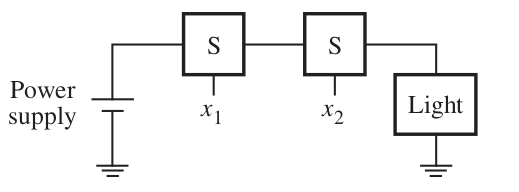
\includegraphics[width=0.2\linewidth]{AND-circuit.png} &
\includegraphics[width=0.2\linewidth]{AND_ANSI.pdf} &
\includegraphics[width=0.2\linewidth]{AND_Venn.pdf}\\
  OR Gate &
\texttt{L = x1 | x2} &
$L = x_1 + x_2$ &
\mbox{\begin{tabular}{cc|c}
  \toprule
  $x_1$ & $x_2$ & $x_1 + x_2$ \\
  \midrule
  0 & 0 & 0 \\
  0 & 1 & 1 \\
  1 & 0 & 1 \\
  1 & 1 & 1 \\
  \bottomrule
\end{tabular}} &
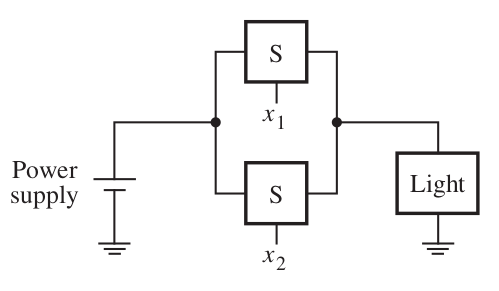
\includegraphics[width=0.2\linewidth]{OR-circuit.png} &
\includegraphics[width=0.2\linewidth]{OR_ANSI.pdf} & 
\includegraphics[width=0.2\linewidth]{OR_Venn.pdf}\\
  NOT Gate &
  \texttt{L = $\sim$ x1} &
$ L = \bar{x}_1 = x'_1$ &
\mbox{\begin{tabular}{c|c}
\toprule
$x_1$ & $\bar{x}_1$ \\
\midrule
0 & 1 \\
1 & 0 \\
\bottomrule
\end{tabular}} &
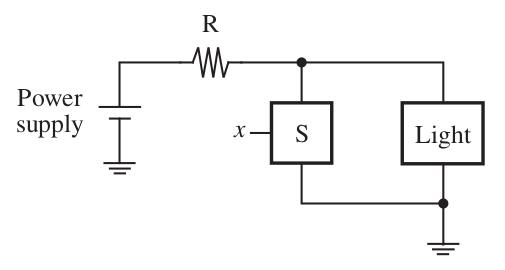
\includegraphics[width=0.2\linewidth]{NOT-circuit.png} &
\includegraphics[width=0.2\linewidth]{NOT_ANSI.pdf} &
\includegraphics[width=0.2\linewidth]{NOT_Venn_x1.pdf}
\end{tabular}
}
\newpage

\section{Digital circuits or networks}

\begin{tikzpicture}[circuit logic US]
    \node (A) at (0,1) {A} ;
    \node (B) at (0,0.5) {B} ;
    \node (C) at (0,0) {C} ;
    \node [draw,rounded corners,inner sep=7mm,anchor=south west] (CL) at (1, -3mm) {CL} ; 
    \node [above right=3mm of CL.east] (Y) {Y} ;
    \node [below right=3mm of CL.east] (Z) {Z} ;

    \draw (A) -| (CL.west);
    \draw (B) -| (CL.west);
    \draw (C) -| (CL.west);
    \draw (CL.east) |- (Y);
    \draw (CL.east) |- (Z);
\end{tikzpicture}

\[
  Y = F(A, B, C) \qquad Z = G(A, B, C)
  \]

\section{Two input networks}
\begin{example}
  Convert the following (ANSI) network into a Boolean expression, a truth table
  and a Venn diagram.

\begin{tikzpicture}[circuit logic US]
  \matrix[column sep=7mm]{
    \node (i1) {$x_1$}; & &  \\
    & \node [and gate] (a) {}; & \node [not gate] (n) {};\\
    \node (i2) {$x_2$}; & &  \\
  };
  \draw (i1.east) -- ++(right:3mm) |- (a.input 1);
  \draw (i2.east) -- ++(right:3mm) |- (a.input 2);
  \draw (a.output) to [edge label=g] (n.input);
  \draw (n.output) to [edge label=f] ++(right:3mm);
\end{tikzpicture}
\end{example}
\vspace{10em}

\begin{example}
  Convert the following Boolean expression into a (ANSI) network, a truth
  table and a Venn diagram:\\
  \[ f = \overline{x_1 + x_2}\]
\end{example}
\vspace{10em}

\begin{prob}[10 marks]
  Convert the following (ANSI) network into a Boolean expression, a truth table
  and a Venn diagram.

 \noindent \begin{tikzpicture}[circuit logic US]
    \matrix[column sep=7mm]{
      \node (i1) {$x_1$}; & & \node [and gate] (x1nx2) {}; & \\
      \node (i2) {$x_2$}; &  &  &  \node [or gate] (f) {}; \\
       & \node [not gate] (n1) {}; & \node [and gate] (nx1x2) {};&  \\
      & \node [not gate] (n2) {}; &  & \\
    };
    \draw (i1.east) -- ++(right:4mm) |- (n1.input);
    \draw (i2.east) -- ++(right:2mm) |- (n2.input);

    \draw (i1.east) -- ++(right:4mm) |- (x1nx2.input 1);
    \draw (i2.east) -- ++(right:2mm) |- (x1nx2.input 2);

    \draw (n1.output) -- ++(right:3mm) |- (nx1x2.input 1);
    \draw (n2.output) -- ++(right:3mm) |- (nx1x2.input 2);

    \draw (x1nx2.output) -- ++(right:3mm) |- (f.input 1);
    \draw (nx1x2.output) -- ++(right:3mm) |- (f.input 2);

    \draw (f.output) to [edge label=f] ++(right:3mm);
  \end{tikzpicture}
\end{prob}
\vspace{10em}

\begin{example}
  Convert the following Boolean expression into a network, a truth
  table and a Venn diagram:\\
  \[ f = x_1 \bar{x}_2 + \bar{x}_1 x_2 \]
\end{example}
\vspace{20em}

\begin{prob}[5 marks]
Can two different circuits have the same truth table? Can two different truth tables
have the same circuit? Consider the following two circuits for example \\
\noindent\begin{tikzpicture}[circuit logic US]
  \node (A) {A}; \node [not gate, right=of A] (notA) {}; \node [right=of notA] (Y) {Y};
  \draw (A) -- (notA.input);
  \draw (notA.output) -- (Y);
\end{tikzpicture}\\[1em]

\noindent\begin{tikzpicture}[circuit logic US]
  \node (A) {A}; \node [not gate, right=of A] (notA1) {};
  \draw (A) -- (notA.input);

  \node [not gate, right=of notA1] (notA2) {};
  \draw (notA1.output) -- (notA2.input);

  \node [not gate, right=of notA2] (notA3) {};
  \draw (notA2.output) -- (notA3.input);

  \node [right=of notA3] (Y) {Y};
  \draw (notA3.output) -- (Y);
\end{tikzpicture}

%How about Venn diagrams?
\end{prob}
\vspace{10em}

\begin{remark}
  Truth tables and Venn diagrams define \emph{what} the combinational circuit should do. Truth tables
  define output for every input.
  Boolean expression and networks define \emph{how} to achieve the desired input
  output relationship.
\end{remark}


\section{Multi-input networks}
\begin{example}
  Convert the following (ANSI) network into a Boolean expression and a truth table.
  \begin{tikzpicture}[circuit logic US]
    \matrix[column sep=7mm]{
      \node (A) {$A$}; & &  \node [and gate] (andAB) {}; & & & \\
      \node (B) {$B$}; & \node [not gate] (nB) {};  &  & \node [or gate] (orGC) {}; & \node [not gate] (notH) {}; & \\
      \node (C) {$C$}; & & \node (C2) {}; & & & \node [and gate] (andHD) {}; \\
      \node (D) {$D$}; & &  & & \node (D2) {}; &\\
    };
    \draw (A) -- ++(right:3mm) |- (andAB.input 1);
    \draw (B) -- (nB.input);
    \draw (nB.output) -- ++(right:3mm) |- (andAB.input 2);

    \draw (andAB.output) to [edge label=g] ++(right:3mm) |- (orGC.input 1);
    \draw (C) -- (C2.east) -- ++(right:3mm) |- (orGC.input 2);

    \draw (orGC.output)  to [edge label=h] (notH.input);

    \draw (notH.output) -- ++(right:3mm) |- (andHD.input 1);
    \draw (D) -- (D2.east) -- ++(right:3mm) |- (andHD.input 2);
    
    \draw (andHD.output) to [edge label=f] ++(right:3mm);
  \end{tikzpicture}
\end{example}
\vspace{20em}

\begin{prob}[20 marks]
  Convert the following (ANSI) network into a Boolean expression and a truth table.
  \begin{tikzpicture}[circuit logic US]
    \matrix[column sep=7mm]{
      \node (A) {$A$}; & &  \node [or gate] (andAB) {}; & & & \\
      \node (B) {$B$}; & \node [not gate] (nB) {};  &  & \node [and gate] (orGC) {}; &  & \\
      \node (C) {$C$}; & & \node (C2) {}; & & & \node [and gate] (andHD) {}; \\
      \node (D) {$D$}; & &  & & \node (D2) {}; &\\
    };
    \draw (A) -- ++(right:3mm) |- (andAB.input 1);
    \draw (B) -- (nB.input);
    \draw (nB.output) -- ++(right:3mm) |- (andAB.input 2);

    \draw (andAB.output) to [edge label=g] ++(right:3mm) |- (orGC.input 1);
    \draw (C) -- (C2.east) -- ++(right:3mm) |- (orGC.input 2);

    %\draw (orGC.output)  to [edge label=h] (andHD.input);

    \draw (orGC.output) to [edge label=h] ++(right:3mm) |- (andHD.input 1);
    \draw (D) -- (D2.east) -- ++(right:3mm) |- (andHD.input 2);
    
    \draw (andHD.output) to [edge label=f] ++(right:3mm);
  \end{tikzpicture}
\end{prob}
\vspace{20em}

\section{Minterms and Maxterms}
\subsection{Minterms}
Minterm is a product involving all inputs (or complements) to a function.
Every row of a truth table has a corresponding minterm.
Minterm is true if and only if the corresponding row in the table is active.

Minterms defined as follows for each row of a two input truth table:\\
\begin{tabular}{rrrp{20mm}}
  \toprule
  A & B &  minterm & minterm name\\
  \midrule
  0 & 0 &  $\bar{A} \bar{B}$ & $m_0$ \\
  0 & 1 &  $\bar{A}      B $ & $m_1$ \\
  1 & 0 &  $     A  \bar{B}$ & $m_2$ \\
  1 & 1 &  $     A       B $ & $m_3$ \\
  \bottomrule
\end{tabular}\\[1em]

\noindent Consider a two input circuit whose output $Y$ is given by the truth table:\\
\begin{tabular}{rrrrp{20mm}}
  \toprule
  A & B &  Y & minterm & minterm name\\
  \midrule
  0 & 0 & 0 & $\bar{A} \bar{B}$ & $m_0$ \\
  0 & 1 & 1 & $\bar{A}      B $ & $m_1$ \\
  1 & 0 & 0 & $     A  \bar{B}$ & $m_2$ \\
  1 & 1 & 1 & $     A       B $ & $m_3$ \\
  \bottomrule
\end{tabular}\\[1em]
then $Y = \bar{A}      B  + A B = m_1 + m_3 = \sum (1, 3)$.

\noindent This also gives the \emph{sum of products canonical form}.

\begin{example}
  What is the minterm $m_{13}$ for a 4-input circuit with inputs $x, y, z, w$
  (ordered from MSB to LSB).
\end{example}
\vspace{10em}

%\noindent Find the minterm $m_n$
%\begin{enumerate}
%    \item Convert the minterm number $n$ to a $m$-bit binary number where $m$ is the
%      order of inputs.
%    \item Replace 0 with the corresponding input complement and 1 with the input.
%\end{enumerate}

\begin{prob}[5 marks]
  What is the minterm $m_{23}$ for a 5-input circuit with inputs $a, b, c, d, e$
  (ordered from MSB to LSB).
\end{prob}
\vspace{10em}

\begin{example}
  Convert the following 4-input truth table into sum of minterms and sum of products canonical form.

  \noindent \begin{tabular}{p{20mm}llll|l}
    \toprule
    minterm name & A & B & C & D & f \\
    \midrule
    $m_0$ & 0 & 0 & 0 & 0 & 0 \\ 
    $m_1$ & 0 & 0 & 0 & 1 & 1 \\ 
    $m_2$ & 0 & 0 & 1 & 0 & 0 \\ 
    $m_3$ & 0 & 0 & 1 & 1 & 0 \\ 
    $m_4$ & 0 & 1 & 0 & 0 & 0 \\ 
    $m_5$ & 0 & 1 & 0 & 1 & 1 \\ 
    $m_6$ & 0 & 1 & 1 & 0 & 0 \\ 
    $m_7$ & 0 & 1 & 1 & 1 & 0 \\ 
    $m_8$ & 1 & 0 & 0 & 0 & 0 \\ 
    $m_9$ & 1 & 0 & 0 & 1 & 0 \\ 
    $m_{10}$ & 1 & 0 & 1 & 0 & 0 \\
    $m_{11}$ & 1 & 0 & 1 & 1 & 0 \\
    $m_{12}$ & 1 & 1 & 0 & 0 & 0 \\
    $m_{13}$ & 1 & 1 & 0 & 1 & 1 \\
    $m_{14}$ & 1 & 1 & 1 & 0 & 0 \\
    $m_{15}$ & 1 & 1 & 1 & 1 & 0 \\
    \bottomrule
  \end{tabular}
\end{example}

\begin{prob}[10 marks]
  Convert the following 4-input truth table into sum of minterms and sum of products canonical form.

  \noindent
  \begin{tabular}{p{20mm}llll|l}
    \toprule
    minterm name & A & B & C & D & f \\
    \midrule
    $m_0$ & 0 & 0 & 0 & 0 & 0 \\ 
    $m_1$ & 0 & 0 & 0 & 1 & 0 \\ 
    $m_2$ & 0 & 0 & 1 & 0 & 0 \\ 
    $m_3$ & 0 & 0 & 1 & 1 & 1 \\ 
    $m_4$ & 0 & 1 & 0 & 0 & 0 \\ 
    $m_5$ & 0 & 1 & 0 & 1 & 0 \\ 
    $m_6$ & 0 & 1 & 1 & 0 & 0 \\ 
    $m_7$ & 0 & 1 & 1 & 1 & 1 \\ 
    $m_8$ & 1 & 0 & 0 & 0 & 0 \\ 
    $m_9$ & 1 & 0 & 0 & 1 & 0 \\ 
    $m_{10}$ & 1 & 0 & 1 & 0 & 0 \\
    $m_{11}$ & 1 & 0 & 1 & 1 & 1 \\
    $m_{12}$ & 1 & 1 & 0 & 0 & 0 \\
    $m_{13}$ & 1 & 1 & 0 & 1 & 1 \\
    $m_{14}$ & 1 & 1 & 1 & 0 & 1 \\
    $m_{15}$ & 1 & 1 & 1 & 1 & 0 \\
    \bottomrule
  \end{tabular}
\end{prob}


\subsection{Maxterms}
Maxterm is a sum involving all inputs (or complements) to a function.
Every row of a truth table has a corresponding maxterm.
Minterm is false if and only if the corresponding row in the table is active.

Maxterms are defined as follows for each row of a two input truth table:\\
\begin{tabular}{rrrp{20mm}}
  \toprule
  A & B &  maxterm & maxterm name\\
  \midrule
  0 & 0 &  $A + B$ & $M_0$ \\
  0 & 1 &  $A + \bar{B} $ & $M_1$ \\
  1 & 0 &  $\bar{A} + B$ & $M_2$ \\
  1 & 1 &  $\bar{A} + \bar{B} $ & $M_3$ \\
  \bottomrule
\end{tabular}\\[1em]

\noindent Consider a two input circuit whose output $Y$ is given by the truth table:\\
\begin{tabular}{rrrrp{20mm}}
  \toprule
  A & B &  Y & maxterm & maxterm name\\
  \midrule
  0 & 0 &  0 & $A + B$ & $M_0$ \\
  0 & 1 &  1 & $A + \bar{B} $ & $M_1$ \\
  1 & 0 &  0 & $\bar{A} + B$ & $M_2$ \\
  1 & 1 &  1 & $\bar{A} + \bar{B} $ & $M_3$ \\
  \bottomrule
\end{tabular}\\[1em]
then $Y = (A+B)(\bar{A} + B) = M_0M_2$.

\noindent Writing a functional specification in terms of minterms is also called
product of sums canonical form.

\begin{example}
  Write the maxterm $M_{11}$ for 4-input Boolean function with the ordered inputs $A, B, C, D$.
\end{example}

% \noindent Find the maxterm $M_n$
% \begin{enumerate}
% \item Convert the maxterm number $n$ to a $m$-bit binary number where $m$ is the
%   order of inputs.
% \item Replace 0 with the corresponding input and 1 with the input complement.
% Add + between each input.
% \end{enumerate}

\begin{example}
  Convert the following 4-input truth table into product of maxterms and product of sums canonical form.

  \noindent
  \begin{tabular}{p{20mm}llll|l}
    \toprule
    maxterm name & A & B & C & D & f \\
    \midrule
    $M_0$ & 0 & 0 & 0 & 0 & 0 \\ 
    $M_1$ & 0 & 0 & 0 & 1 & 0 \\ 
    $M_2$ & 0 & 0 & 1 & 0 & 0 \\ 
    $M_3$ & 0 & 0 & 1 & 1 & 1 \\ 
    $M_4$ & 0 & 1 & 0 & 0 & 0 \\ 
    $M_5$ & 0 & 1 & 0 & 1 & 0 \\ 
    $M_6$ & 0 & 1 & 1 & 0 & 0 \\ 
    $M_7$ & 0 & 1 & 1 & 1 & 1 \\ 
    $M_8$ & 1 & 0 & 0 & 0 & 0 \\ 
    $M_9$ & 1 & 0 & 0 & 1 & 0 \\ 
    $M_{10}$ & 1 & 0 & 1 & 0 & 0 \\
    $M_{11}$ & 1 & 0 & 1 & 1 & 1 \\
    $M_{12}$ & 1 & 1 & 0 & 0 & 0 \\
    $M_{13}$ & 1 & 1 & 0 & 1 & 1 \\
    $M_{14}$ & 1 & 1 & 1 & 0 & 1 \\
    $M_{15}$ & 1 & 1 & 1 & 1 & 0 \\
    \bottomrule
  \end{tabular}
\end{example}

\begin{prob}[10 marks]
  Convert the following 4-input truth table into product of maxterms and products of sums canonical form.

  \noindent
  \begin{tabular}{p{20mm}llll|l}
    \toprule
    maxterm name & A & B & C & D & f \\
    \midrule
    $M_0$ & 0 & 0 & 0 & 0 & 0 \\ 
    $M_1$ & 0 & 0 & 0 & 1 & 1 \\ 
    $M_2$ & 0 & 0 & 1 & 0 & 1 \\ 
    $M_3$ & 0 & 0 & 1 & 1 & 1 \\ 
    $M_4$ & 0 & 1 & 0 & 0 & 1 \\ 
    $M_5$ & 0 & 1 & 0 & 1 & 0 \\ 
    $M_6$ & 0 & 1 & 1 & 0 & 1 \\ 
    $M_7$ & 0 & 1 & 1 & 1 & 1 \\ 
    $M_8$ & 1 & 0 & 0 & 0 & 0 \\ 
    $M_9$ & 1 & 0 & 0 & 1 & 1 \\ 
    $M_{10}$ & 1 & 0 & 1 & 0 & 1 \\
    $M_{11}$ & 1 & 0 & 1 & 1 & 1 \\
    $M_{12}$ & 1 & 1 & 0 & 0 & 0 \\
    $M_{13}$ & 1 & 1 & 0 & 1 & 1 \\
    $M_{14}$ & 1 & 1 & 1 & 0 & 1 \\
    $M_{15}$ & 1 & 1 & 1 & 1 & 0 \\
    \bottomrule
  \end{tabular}
\end{prob}

\begin{example}
  Write the 3-input truth table for the function $f = m_2 + m_3 + m_7$.
\end{example}
\vspace{10em}

\begin{prob}[10 marks]
  Write the 3-input truth table for the function $f = M_4M_5M_7$. 
\end{prob}
\vspace{10em}

\begin{prob}[10 marks]
  Write the truth table for the function $f = \bar{A}B\bar{C} + AB\bar{C}$. 
\end{prob}
\vspace{10em}
